
%% ==================================================================================================
%%
\documentclass[12pt]{book}
\usepackage{amsfonts}
\usepackage{amsmath}
\usepackage{amssymb}
\usepackage{graphicx}
\usepackage{hyperref}
\usepackage{float}
\usepackage{verbatim}
\usepackage{xlop} %% for multiplication https://tex.stackexchange.com/questions/11702/how-to-present-a-vertical-multiplication-addition
\usepackage{listings} %% to format generic computer code
\usepackage{lmodern} % for bold teletype font
\usepackage{minted} % colour Java code


\usepackage{tasks}
%\NewTasks[style=enumerate,counter-format=tsk[A].,label-width=3ex]{choice}[\item](4)

%% =======   set page margins    =======
\setlength{\textheight}{10in}
\setlength{\textwidth}{7.4in}
\setlength{\topmargin}{-0.75in}
\setlength{\oddsidemargin}{-0.5in}
\setlength{\evensidemargin}{-0.5in}
\setlength{\parskip}{0.15in}
\setlength{\parindent}{0in}

%%  for European long division
% https://tex.stackexchange.com/questions/432435/how-to-set-up-european-french-style-long-division-in-tex
\newcommand\frdiv[5]{%
    \[
    \renewcommand\arraystretch{1.5}
    \begin{array}{l| l}
    #1 & #2 \\
    \cline{2-2}
    #3 & #4 \\
    \cline{1-1}
    #5 & \\
    \end{array}
    \]
}

%%  for European long division


%% ==================================================================================================

\begin{document}

%\title{ITI1100 Digital Systems I}
%\author{Kien Do 300163370}
%\date{Assignment \#1}
\newcommand{\reporttitle}{Devoir 8: Graphe}
\newcommand{\reportauthorOne}{Kien Do}
\newcommand{\cidOne}{300163370}
\input{titlePage/titlepage.txt}



%% ==================================================================================================

%%%%%%%%%%%% PROBLEMS START HERE

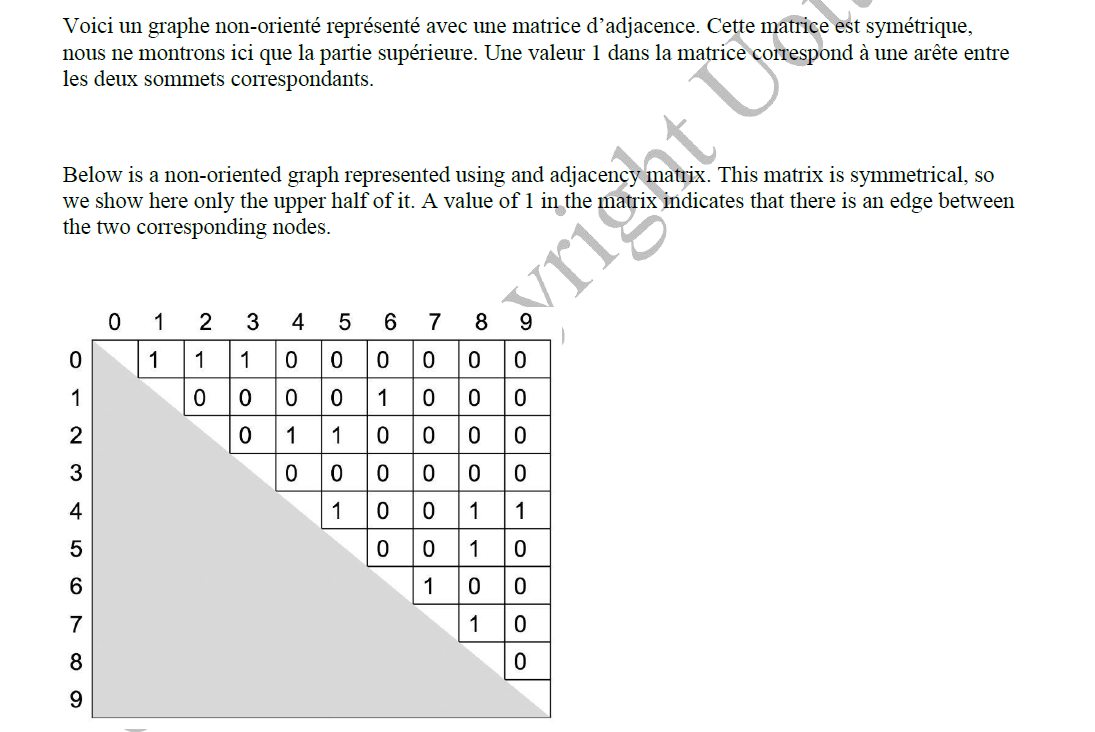
\includegraphics[scale=0.80]{graphQuestion.png}\\

\begin{enumerate}
    
    \item Dessiner le graphe correspondant à cette matrice.\\
    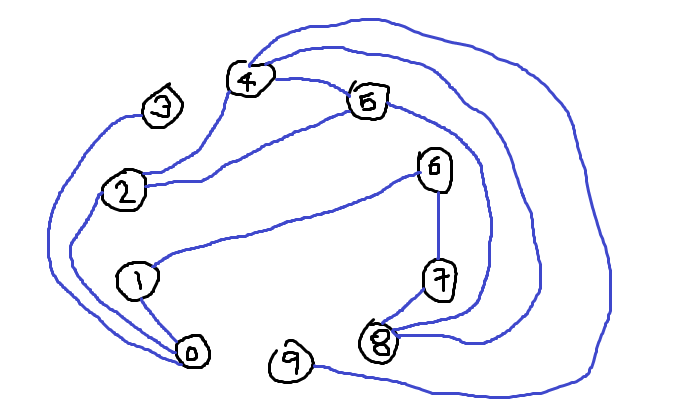
\includegraphics[scale=0.80]{d8a1.png}
    
    \newpage
    
    \item Remplacer cette représentation avec matrice d’adjacence pour une représentation avec listes d’adjacence. Chacune des arêtes dans les listes d’adjacence doit être identifiée comme suit : \\
    \hspace*{10mm} \textbf{0-1} pour l’arête liant le noeud 0 au noeud 1.\\
    Ordonner les arêtes en suivant l’ordre de gauche à droite dans les rangées de la matrice.\\
    
    0: (0-1), (0-2), (0-3)\\
    1: (1-0), (1-6)\\
    2: (2-0), (2-4), (2-5)\\
    3: (3-0)\\
    4: (4-2), (4-5), (4-8), (4-9)\\
    5: (5-2), (5-4), (5-8)\\
    6: (6-1), (6-7)\\
    7: (7-6), (7-8)\\
    8: (8-4), (8-5), (8-7)\\
    9: (9-4)\\
    
    \item Effectuer une traversée en profondeur de ce graphe à partir du noeud 0 en utilisant une pile tel que vu en classe. Lorsque les arêtes sont empilées, toujours suivre l’ordre de gauche à droite comme pour la ques- tion 2 (par exemple pour le sommet 2, l’arête 2-4 sera empilée avant l’arête 2-5). Bien montrer l’état de la pile après chaque visite de sommet. Donner aussi, dans l’ordre, les arêtes de l’arbre T utilisées pour passer d’un noeud courant au prochain noeud non-exploré.
    %% $\xleftarrow[]{}$ (0-2) $\xleftarrow[]{}$ (0-3)
    \begin{tabbing}
    
    Visited: \{0\} \hspace{10em} \= to visit \hspace{1em} \= 
        \begin{tabular}{ |c| }
        0-3 \\ 
        0-2 \\  
        0-1 \\
        \hline
        \end{tabular}
    \\\\
    
    POP $\xrightarrow[]{}$ (0-3)\\Visited: \{0,3,2\}\\T=\{(0-3),(0-2)\} \> to visit \>  
        \begin{tabular}{ |c| } 
        0-2 \\  
        0-1 \\
        \hline
        \end{tabular}
    \\\\
    
    POP $\xrightarrow[]{}$ (0-2)\\Visited: \{0,3,2\}\\T=\{(0-3),(0-2)\} \> to visit \>  
        \begin{tabular}{ |c| } 
        2-5\\
        2-4 \\
        0-1 \\
        \hline
        \end{tabular}
    \\\\
    
    POP $\xrightarrow[]{}$ (2-5)\\Visited: \{0,3,2,5\}\\T=\{(0-3),(0-2),(2-5)\} \> to visit \>  
        \begin{tabular}{ |c| } 
        5-8 \\
        5-4 \\
        2-4 \\
        0-1 \\
        \hline
        \end{tabular}
    \\\\
    
    POP $\xrightarrow[]{}$ (5-8)\\Visited: \{0,3,2,5,8\}\\T=\{(0-3),(0-2),(2-5),(5-8)\} \> to visit \>  
        \begin{tabular}{ |c| }
        8-7\\
        8-4\\
        5-4 \\
        2-4 \\
        0-1 \\
        \hline
        \end{tabular}
    \\\\
    
    POP $\xrightarrow[]{}$ (8-7)\\Visited: \{0,3,2,5,8,7\}\\T=
    \[
        \left\{
        \begin{tabular}{c}
        (0-3),(0-2),(2-5),(5-8),\\
        (8-7)
        \end{tabular}
        \right\}
    \]
    \> to visit \>  
        \begin{tabular}{ |c| }
        7-6\\
        8-4\\
        5-4 \\
        2-4 \\
        0-1 \\
        \hline
        \end{tabular}
    \\\\
    
    POP $\xrightarrow[]{}$ (7-6)\\Visited: \{0,3,2,5,8,7,6\}\\T=
    \[
        \left\{
        \begin{tabular}{c}
        (0-3),(0-2),(2-5),(5-8),\\
        (8-7),(7-6)
        \end{tabular}
        \right\}
    \]
    \> to visit \>  
        \begin{tabular}{ |c| }
        6-1\\
        8-4\\
        5-4 \\
        2-4 \\
        0-1 \\
        \hline
        \end{tabular}
    \\\\
    
    POP $\xrightarrow[]{}$ (6-1)\\Visited: \{0,3,2,5,8,7,6,1\}\\T=
    \[
        \left\{
        \begin{tabular}{c}
        (0-3),(0-2),(2-5),(5-8),\\
        (8-7),(7-6),(6-1)
        \end{tabular}
        \right\}
    \]
    \> to visit \>  
        \begin{tabular}{ |c| }
        8-4\\
        5-4 \\
        2-4 \\
        0-1 \\
        \hline
        \end{tabular}
    \\\\
    
    POP $\xrightarrow[]{}$ (8-4)\\Visited: \{0,3,2,5,8,7,6,1,4\}\\T=
    \[
        \left\{
        \begin{tabular}{c}
        (0-3),(0-2),(2-5),(5-8),\\
        (8-7),(7-6),(6-1),(8-4)
        \end{tabular}
        \right\}
    \]
    \> to visit \>  
        \begin{tabular}{ |c| }
        4-9\\
        5-4 \\
        2-4 \\
        0-1 \\
        \hline
        \end{tabular}
    \\\\
    
    POP $\xrightarrow[]{}$ (4-9)\\Visited: \{0,3,2,5,8,7,6,1,4,9\}\\\\T=
    \[
        \left\{
        \begin{tabular}{c}
        (0-3),(0-2),(2-5),(5-8),\\
        (8-7),(7-6),(6-1),(8-4),\\
        (4-9)
        \end{tabular}
        \right\}
    \]
    \> to visit \>  
        \begin{tabular}{ |c| }
        5-4 \\
        2-4 \\
        0-1 \\
        \hline
        \end{tabular}
    
    \end{tabbing}
    
    L'algorithme s'arrête ici car le nombre de noeuds visités est égal au nombre total de noeuds (cela veut dire que tous les noeuds ont été visités et la traversée est terminée).
    
    \newpage
    
    \item Utilisant l’algorithme ci-dessous, effectuer une traversée en largeur du graphe en partant du noeud 0. Dessiner le graphe en identifiant les arêtes DISCOVERY et CROSS. Lister les sommets dans l’ordre de visite en encerclant les groupes correspondants aux listes: L\_0, L\_1, L\_2,…
    
    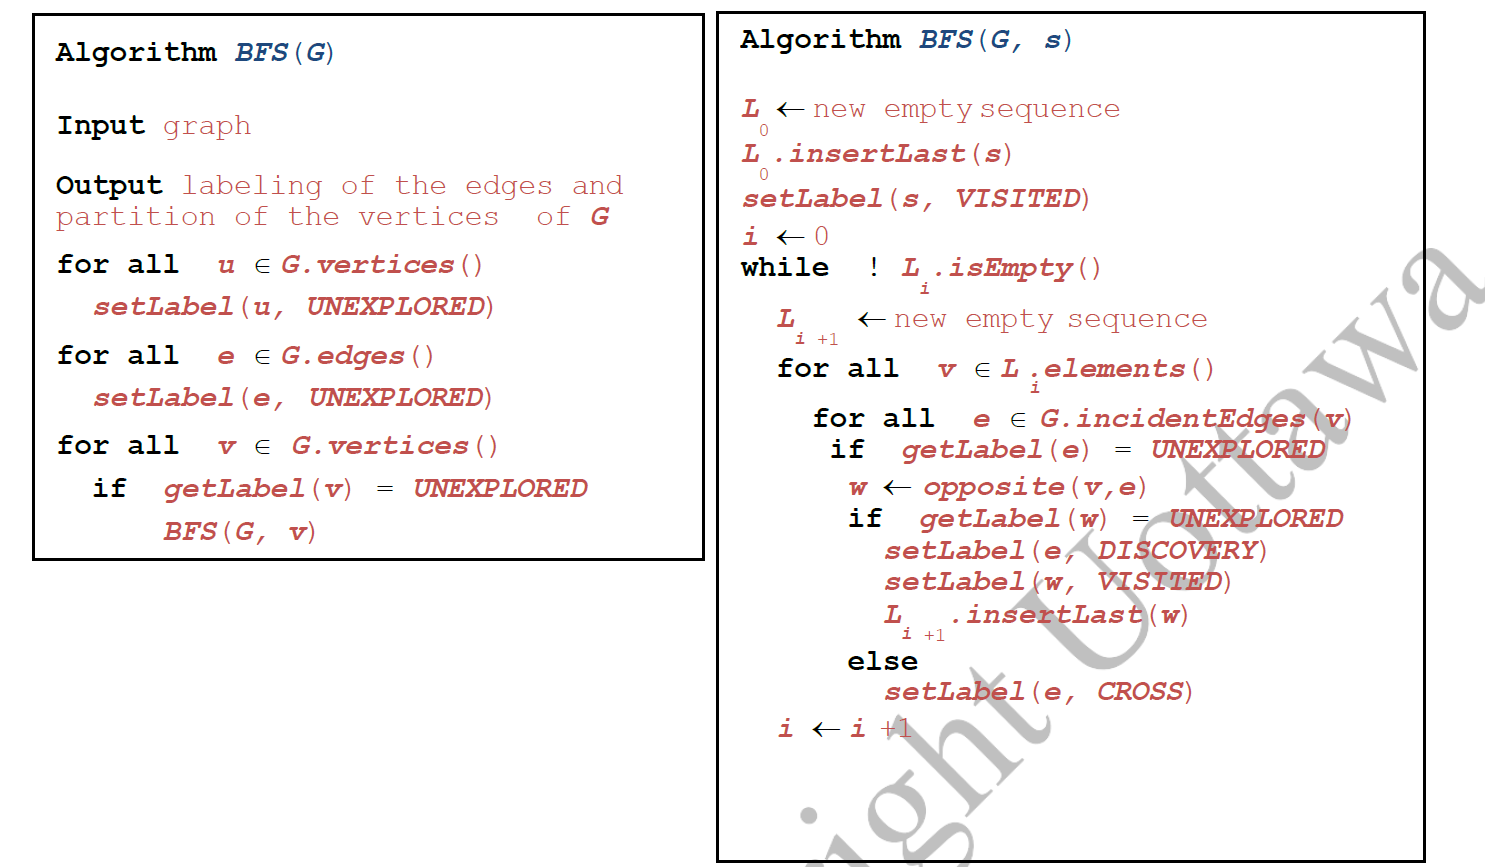
\includegraphics[scale=0.50]{d8q4BFSalgorithms.png}\\
    
    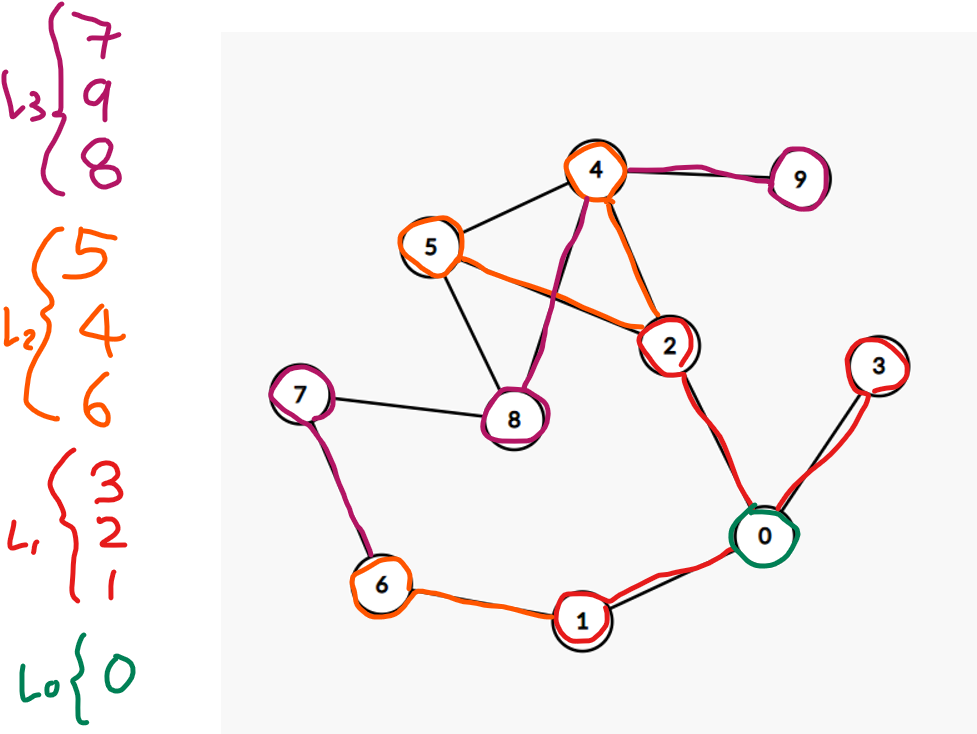
\includegraphics[scale=0.70]{d8a4.png}\\
    
    
\end{enumerate}





\end{document} 
